% N-a-002: original Fraisse1954 presentation and explicit modern consequences.
\chapter{Ages, Amalgamation, and Homogeneous Relations}
\label{sec:p03-fraisse-1954}

A collection of finite configurations need not determine a unique infinite
structure. Two separate questions arise: whether it is the age of a structure,
and whether it has a homogeneous representative. Fra\"iss\'e's original
argument answers these questions by different conditions. It also constructs
relations on arbitrary bases through filters of maps
\cite[\S\S1--10, pp.~363--388]{Fraisse1954}.
We first develop that single-relation presentation. The final sections give
the countable-signature extension and the simple-graph consequences, with
their proofs supplied explicitly.
The ambient set theory is ZFC. Classes in the metatheorems are definable
classes of set-based relations, and input families are set indexed.
The ultrafilter and transfinite constructions state where these assumptions
enter.

\section{Relations, restrictions, and finite configurations}
\label{sec:p03-fraisse54-relations}

\begin{hbdefinition}{def:p03-fraisse54-relation}{A relation and its embeddings}
Fix a positive integer \(n\). An \(n\)-ary relation on a set \(E\) is a
function \(R:E^n\to\{+,-\}\). Empty bases are allowed. Its restriction to
\(D\subseteq E\) is \(R\mathbin{\upharpoonright}D:D^n\to\{+,-\}\).
An embedding \(f:A\to B\) is an injection between the bases satisfying
\[
 A(a_1,\ldots,a_n)=B(f(a_1),\ldots,f(a_n))
\]
for every tuple, including tuples with repeated entries. Thus it preserves
both positive and negative instances. A surjective embedding is an
isomorphism, and an isomorphism from a relation to itself is an automorphism.
Transport along a bijection defines a copy of a relation on a new base.
Its isomorphism type is the class of all its isomorphic copies.
A chain is a set-indexed family whose bases are linearly ordered
by inclusion and in which the relation on every larger base restricts to
the relation on every smaller base.
These are the relational conventions of \cite[\S1.2]{Fraisse1954}.
\index{embedding!relational}\index{relation!two-valued}
\end{hbdefinition}

\begin{hbdefinition}{def:p03-fraisse54-age}{Embedding preorders, ages, and local closure}
Write \(A\ll B\) when an embedding \(A\to B\) exists, and
\(A\prec B\) when every finite restriction of \(A\) embeds into \(B\).
The \emph{age} \(\gamma_R\) is the isomorphism-closed class of finite
relations embedding into \(R\). Put
\[
 \Gamma_R=\{A:A\prec R\}.
\]
These are classes of structures in the metalanguage. In particular,
\(\gamma_R\) consists exactly of the finite members of \(\Gamma_R\).
The notation retains the two different comparisons in
\cite[\S\S1.3--1.4]{Fraisse1954}.
\index{age of a structure}\index{local embeddability}
\end{hbdefinition}

\begin{hblemma}{thm:p03-fraisse54-basic}{proved=annex:p3.fraisse54.basic}{Restriction, transport, and comparison}
The relations \(\ll\) and \(\prec\) are reflexive, transitive and
isomorphism invariant; \(A\ll B\) implies \(A\prec B\). A chain of
compatible restrictions has a unique union relation. A bijection is an
isomorphism if its restrictions to sets of at most \(n\) elements are
isomorphisms. Neither mutual finite embeddability nor mutual embeddability
implies isomorphism in general. For orders, adjoining or deleting the
diagonal translates between reflexive and strict presentations without
changing induced embeddings or automorphisms.
The classes \(\Gamma_R\) are determined by their finite members. If
\(R\in\mathcal K=\Gamma_S\), then \(\Gamma_R=\mathcal K\) exactly
when every finite member of \(\mathcal K\) embeds into \(R\).
\end{hblemma}

\begin{hbdefinition}{def:p03-fraisse54-closures}{Three closure conditions}
For a nonempty class \(\mathcal K\) of relations, use the following conditions:
\begin{enumerate}
\item \(\mathrm C_1\): closure under isomorphism and restriction;
\item \(\mathrm C_2\): any two members embed into a common member;
\item \(\mathrm C_3\): the union of any nonempty chain of compatible
      members is a member.
\end{enumerate}
On finite relations, \(\mathrm C_1\) is the hereditary property and
\(\mathrm C_2\) is the joint-embedding property. They do not assert
amalgamation over an already identified common part.
\end{hbdefinition}

\begin{hbtheorem}{thm:p03-fraisse54-age-count}{proved=annex:p3.fraisse54.age-count}{How many single-relation ages exist?}
For a fixed positive arity, there are countably many finite isomorphism types.
There are exactly countably infinitely many ages of unary relations, and
exactly \(2^{\aleph_0}\) ages of \(n\)-ary relations for every \(n\geq2\).
The same counts hold for the associated classes \(\Gamma_R\).
\end{hbtheorem}

\begin{hblemma}{thm:p03-fraisse54-chain-hosts}{proved=annex:p3.fraisse54.chain-hosts}{Arranging joint hosts in a chain}
Let \(\mathcal K\) be an isomorphism-closed class with joint embedding.
Every finite or countable family in \(\mathcal K\) admits a chain of
members such that each original member embeds into a stage. If
\(\mathcal K\) is also closed under chain unions, the same conclusion
holds for every set-indexed family, in set theory with Choice.
\end{hblemma}

\begin{hbtheorem}{thm:p03-fraisse54-age-realization}{proved=annex:p3.fraisse54.age-realization}{Realizing an age without amalgamation}
A nonempty class of finite \(n\)-ary relations is an age if and only if it
satisfies \(\mathrm C_1\) and \(\mathrm C_2\). It has a finite or countable
representative. A nonempty inclusion-chain of ages has both its union and
its intersection as ages.
\end{hbtheorem}

This is Theorem II of \cite[\S\S2.3--2.7]{Fraisse1954}. It constructs a
representative of the finite configurations; homogeneity requires the
additional extension conditions developed below.

\section{Projection filters and relations on arbitrary bases}
\label{sec:p03-fraisse54-projection-filters}

\begin{hbdefinition}{def:p03-fraisse54-projection}{Projection filters}
Let \(E,D\) be sets with \(D\ne\varnothing\), and let
\(X=D^E\) be the set of all maps \(E\to D\). A projection filter is a
proper filter \(\mathcal F\) on \(X\): it contains \(X\), is upward
closed and finite-intersection closed, and omits the empty set.
An ultrafilter is a proper filter containing exactly one of
\(Y,X\setminus Y\) for each \(Y\subseteq X\).
For a relation \(R\) on \(D\), a relation \(A\) on \(E\) is its inverse
projection through \(\mathcal F\) when, for each \(\bar a\in E^n\),
\[
 \{f\in X:R(f\bar a)=A(\bar a)\}\in\mathcal F.
\]
When it exists, write \(A=\mathcal F^{-1}(R)\). A single map gives the
ordinary inverse-image relation and its principal projection filter.
For \(H\subseteq E\), the restriction \(\mathcal F_H\) is the direct
image of the filter under \(f\mapsto f|H\).
The filter is \emph{normal} when it contains
\[
 I_H=\{f\in X:f|H\hbox{ is injective}\}
\]
for every finite \(H\subseteq E\). Here normality concerns finite
injectivity; it is not normality of a measure on a cardinal.
An inverse-image relation under a surjection onto its image is called a
\emph{polymorph} in the source; injectivity is an additional condition.
\index{projection filter}\index{normality!projection filter}
\end{hbdefinition}

\begin{hblemma}{thm:p03-fraisse54-filter-calculus}{proved=annex:p3.fraisse54.filter-calculus}{Projection-filter calculus}
An inverse projection through a proper filter is unique when it exists.
It exists through every ultrafilter. Refining a filter preserves an existing
inverse projection, and restricting the filter restricts that relation.
Restrictions of ultrafilters are ultrafilters. Normality is preserved by
refinement and restriction, and normal projection filters \(E\to D\)
exist whenever \(D\) is infinite.
\end{hblemma}

\begin{hbdefinition}{def:p03-fraisse54-filter-equality}{Equality through a projection filter}
For \(a,b\in E\), put
\[
 a\sim_{\mathcal F}b
 \quad\Longleftrightarrow\quad
 \{f\in D^E:f(a)=f(b)\}\in\mathcal F.
\]
This equivalence relation concerns equality of images on a filter-large set
of maps. It is different from equality in the base \(E\).
\end{hbdefinition}

\begin{hblemma}{thm:p03-fraisse54-filter-equality}{proved=annex:p3.fraisse54.filter-equality}{Equality, normality, and transport}
The relation \(\sim_{\mathcal F}\) is an equivalence relation and restricts
with the filter. A normal filter identifies no distinct base elements.
For an ultrafilter, the converse holds. If
\(A=\mathcal F^{-1}(R)\), \(H\subseteq E\), and
\(g:H\to g[H]\subseteq E\) is a bijection satisfying
\(a\sim_{\mathcal F}g(a)\) for all \(a\in H\), then \(g\) is an
isomorphism between the corresponding restrictions of \(A\).
\end{hblemma}

\begin{hbtheorem}{thm:p03-fraisse54-local-projection}{proved=annex:p3.fraisse54.local-projection}{Finite information and projection filters}
Let \(R\) have nonempty base \(D\), and let \(A\) have base \(E\).
An inverse projection \(A=\mathcal F^{-1}(R)\) exists for some filter
\(\mathcal F\) if and only if every finite restriction of \(A\) is the
inverse image of a restriction of \(R\) under a surjective map onto its
image. A normal such filter exists if and only if \(A\prec R\).
In either case an ultrafilter refinement may be used.
\end{hbtheorem}

\begin{hbtheorem}{thm:p03-fraisse54-gamma}{proved=annex:p3.fraisse54.gamma}{Local classes, chains, and common extensions}
In set theory with Choice:
\begin{enumerate}
\item A nonempty class is some \(\Gamma_R\) if and only if it satisfies
      \(\mathrm C_1,\mathrm C_2,\mathrm C_3\).
\item Either \(\Gamma_R\) is generated by one finite relation and its
      restrictions, or it has a member on every set as base.
\item Every set-indexed family of members of \(\Gamma_R\) embeds into
      one common member of \(\Gamma_R\).
\end{enumerate}
These are the two clauses of original Theorem III and Theorem IV
\cite[\S4]{Fraisse1954}. Part 3 has no countability conclusion.
\end{hbtheorem}

\section{Homogeneity and finite extension}
\label{sec:p03-fraisse54-homogeneity}
\begin{hbdefinition}{def:p03-fraisse54-universal}{The countable universality condition}
The source's condition \(\mathcal C\) for a local class \(\mathcal K\)
means that it has a finite or countable member \(U\) such that every finite
or countable member of \(\mathcal K\) embeds into \(U\).
It requires one host of controlled size. The arbitrary-family host theorem
alone does not impose that size bound \cite[\S4.7]{Fraisse1954}.
\end{hbdefinition}

\begin{hbdefinition}{def:p03-fraisse54-extension}{Homogeneity and condition \(\mathcal H\)}
A relation \(R\) is homogeneous when every isomorphism between finite
restrictions of \(R\) extends to an automorphism of \(R\).
Condition \(\mathcal H\) says that whenever \(A\subseteq B\) are finite
relations in \(\gamma_R\), every embedding \(A\to R\) extends to an
embedding \(B\to R\). Restricting this requirement to one-point extensions
gives the same condition.
The source's homogeneous relation is the ultrahomogeneous relational
structure of \cref{def:p03-ultrahomogeneous}; it concerns finite structural
maps, not partial elementary maps.
\end{hbdefinition}

\begin{hbtheorem}{thm:p03-fraisse54-extension}{proved=annex:p3.fraisse54.extension}{Extension, universality, and back-and-forth}
\begin{enumerate}
\item Every homogeneous relation satisfies \(\mathcal H\).
\item If \(R\) satisfies \(\mathcal H\), every finite or countable
      \(A\prec R\) embeds into \(R\).
\item If finite or countable \(R,S\) both satisfy \(\mathcal H\) and
      have the same age, every finite partial isomorphism between them
      extends to an isomorphism \(R\to S\).
\item On finite or countable bases, \(\mathcal H\) is equivalent to
      homogeneity.
\end{enumerate}
The target in part 2 need not be countable. Countability in parts 3--4
cannot simply be removed \cite[\S5]{Fraisse1954}.
\end{hbtheorem}

\section{Amalgamation and the original finite-stage construction}
\label{sec:p03-fraisse54-amalgamation}

\begin{hbdefinition}{def:p03-fraisse54-amalgamation}{Three amalgamation conditions}
For an isomorphism-closed class of finite relations, \(\mathcal D\)
requires amalgamation of every pair of embeddings with a common domain.
Equivalently, \(\mathcal D'\) requires extending an embedding of a
restriction of \(A\) into \(B\) to an embedding of all of \(A\) into
an extension of \(B\). The stronger condition
\(\overline{\mathcal D}\) requires a common extension of the actual
relations \(A,B\) whenever they agree on the intersection of their bases:
no additional identifications of distinct base elements are permitted.
These are the three separately defined conditions of
\cite[\S7.1]{Fraisse1954}.
\index{amalgamation property}\index{strong amalgamation}
\end{hbdefinition}

\begin{hblemma}{thm:p03-fraisse54-amalgamation}{proved=annex:p3.fraisse54.amalgamation}{Amalgamation forms and finite batches}
The conditions \(\mathcal D\) and \(\mathcal D'\) are equivalent.
The condition \(\overline{\mathcal D}\) implies them and is strictly
stronger, even for the finite members of a class \(\Gamma_R\).
Under \(\mathcal D\), any finite list of finite extension problems over
one finite relation can be solved in a common finite extension.
\end{hblemma}

\begin{hbtheorem}{thm:p03-fraisse54-original-construction}{proved=annex:p3.fraisse54.original-construction}{Fra\"iss\'e's single-relation construction}
Let \(\mathcal K=\Gamma_A\), with a fixed positive finite arity.
There is a homogeneous \(R\) with \(\Gamma_R=\mathcal K\) if and only
if the finite members of \(\mathcal K\) have \(\mathcal D\).
When this holds, one such \(R_0\) is finite or countable, is unique up to
isomorphism among finite or countable such relations, and embeds into every
homogeneous \(R\) with \(\Gamma_R=\mathcal K\).
Every finite or countable member of \(\mathcal K\) embeds into \(R_0\).
\end{hbtheorem}

The source's schedule is finite at each stage. At stage \(p\), it treats
all isomorphism types of at most \(p\) elements and all relevant embeddings
of their restrictions into the preceding stage. Finiteness follows from
the one-relation, fixed-arity signature. The annex proves that an extension
problem appearing late in the union is nevertheless scheduled; enumerating
only the structures would not establish this point
\cite[\S\S8.1--8.5]{Fraisse1954}.

\section{Orders, amalgams, and failure cases}
\label{sec:p03-fraisse54-examples}

The source encodes orders by their reflexive relations. We use
\(x<y\) for \(x\leq y\) and \(x\ne y\), particularly in the diagrams
and order-type examples. The diagonal translation of
\cref{thm:p03-fraisse54-basic} identifies their embeddings precisely.

\begin{hbtheorem}{thm:p03-fraisse54-examples}{proved=annex:p3.fraisse54.examples}{The original relation and order examples}
The classes of all \(n\)-ary relations, all linear orders, and all partial
orders satisfy the local-class conditions and
\(\overline{\mathcal D}\) on finite members. Each has a unique countable
homogeneous representative of its full finite age, universal for its
countable members. The class of ramified partial orders, in which the
predecessors of every element form a chain, is a local class but fails
\(\mathcal D\). It therefore has no homogeneous representative of its
full finite age.
\end{hbtheorem}

\begin{figure}[htbp]
\centering
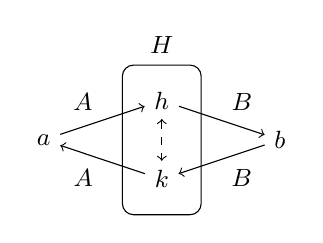
\begin{tikzpicture}[every node/.style={font=\small}]
\draw[rounded corners] (1.0,-.45) rectangle (2.0,1.45);
\node at (1.5,1.7) {$H$};
\node (fa) at (0,.5) {$a$}; \node (fh) at (1.5,1) {$h$};
\node (fb) at (3,.5) {$b$}; \node (fk) at (1.5,0) {$k$};
\draw[->] (fa)--node[above left] {$A$}(fh);
\draw[->] (fh)--node[above right] {$B$}(fb);
\draw[->] (fb)--node[below right] {$B$}(fk);
\draw[->] (fk)--node[below left] {$A$}(fa);
\draw[<->,dashed] (fh)--(fk);
\end{tikzpicture}
\caption{The cross-side cycle in a partial-order amalgam. Solid arrows are
the assumed weak comparisons, labeled by their original order.
Their composites force \(h\leq k\) and \(k\leq h\) inside the common
part \(H\), and then force \(a=h\), contrary to \(a\notin H\).
The relational data are those of \cite[Fig.~1, p.~386]{Fraisse1954}.}
\label{fig:p03-fraisse54-order-cycle}
\end{figure}

\begin{figure}[htbp]
\centering
\begin{tikzpicture}[scale=.9, every node/.style={font=\small}]
\node (a) at (0,1.6) {$a$}; \node (b) at (1.1,1.6) {$b$};
\node (c) at (2.2,1.6) {$c$}; \node (d) at (.55,0) {$d$};
\draw[->] (d)--(a); \draw[->] (d)--(b);
\node at (1.1,-.65) {$A$};
\node (aa) at (4,1.6) {$a$}; \node (bb) at (5.1,1.6) {$b$};
\node (cc) at (6.2,1.6) {$c$}; \node (e) at (5.65,0) {$e$};
\draw[->] (e)--(bb); \draw[->] (e)--(cc);
\node at (5.1,-.65) {$B$};
\node (aaa) at (8,1.6) {$a$}; \node (bbb) at (9.1,1.6) {$b$};
\node (ccc) at (10.2,1.6) {$c$};
\node (dd) at (8.7,-.2) {$d'$}; \node (ee) at (9.5,.5) {$e'$};
\draw[->] (dd)--(aaa); \draw[->] (dd)--(ee);
\draw[->] (ee)--(bbb); \draw[->] (ee)--(ccc);
\draw[->,dashed] (dd) to[bend right=20] (ccc);
\node at (9.1,-.85) {$d'<e'\text{ case}$};
\end{tikzpicture}
\caption{The ramified-order obstruction. Arrows show strict order;
reflexive pairs are implicit. The common base is the antichain
\(\{a,b,c\}\). An amalgam would have to compare the two predecessors of
\(b\), forcing a new comparison inside \(A\) or \(B\).
The dashed comparison in the displayed case contradicts the embedding of
\(A\); the reverse comparison gives the symmetric contradiction in \(B\).
Coincident images of \(d,e\) also force a forbidden comparison.
This redraws the relational data of \cite[Fig.~2, p.~387]{Fraisse1954}.}
\label{fig:p03-fraisse54-ramified}
\end{figure}

\begin{hbtheorem}{thm:p03-fraisse54-orders}{proved=annex:p3.fraisse54.orders}{Homogeneous orders and the countability boundary}
Initial and final segments here mean the strict segments below and above
a specified point; open intervals have two distinct endpoints in increasing
order.
A linear order is homogeneous exactly when its initial segments, final
segments and open intervals have types independent of their
chosen endpoints within each of these three families. For an order with
at least two elements, \(\mathcal H\) is equivalent to density and absence
of endpoints. Consequently the only nontrivial countable homogeneous order
is \((\mathbb Q,<)\).
There are uncountable homogeneous orders of different types, whereas
\(\mathbb R\setminus\{0\}\) satisfies \(\mathcal H\) and is not homogeneous.
\end{hbtheorem}

The source also asks about a merely universal countable ramified order.
Failure of amalgamation rules out a homogeneous representative of the full
age; it does not by itself rule out a countable universal host. These are
the separate questions distinguished in \cite[\S\S4.7, 9.5]{Fraisse1954}.

\section{The explicit countable-signature bridge}
\label{sec:p03-fraisse54-modern}

\begin{hbtheorem}{thm:p03-fraisse54-countable-language}{proved=annex:p3.fraisse54.countable-language}{Fra\"iss\'e limits in a countable relational signature}
Let \(\tau\) be a countable signature of relations of finite arity, with
no function or constant symbols. Let \(\mathcal K\) be a nonempty,
isomorphism-closed class of finite \(\tau\)-structures with countably many
isomorphism types and unbounded finite sizes. Then \(\mathcal K\) is the
age of a countably infinite ultrahomogeneous structure if and only if it
has the hereditary, joint-embedding and amalgamation properties.
The structure is unique up to isomorphism and is universal, by induced
embeddings, for countable structures whose age is contained in \(\mathcal K\).
\end{hbtheorem}

The proof uses an enumeration of finite structures and, at every stage,
the finitely many embeddings of finitely many enumerated structures into
the current stage. It does not assume that a countable signature has only
finitely many structures of a given finite size. In this theorem the age
itself must have countably many types. The original fixed-arity proof and
this enumeration are thus two explicit schedules for the same extension task.

\begin{hbtheorem}{thm:p03-fraisse54-categoricity-boundary}{proved=annex:p3.fraisse54.categoricity-boundary}{Finite signatures and a countable-signature counterexample}
In a finite relational signature with no function or constant symbols,
a countably infinite ultrahomogeneous
structure has quantifier elimination in its complete theory and is
\(\aleph_0\)-categorical. Empty conjunctions and disjunctions may be used
as logical truth and falsity in the quantifier-free language.
The corresponding claim for all countable relational signatures is false,
even for a Fra\"iss\'e class with countably many finite types and amalgamation.
\end{hbtheorem}

\section{The simple-graph interface}
\label{sec:p03-fraisse54-graph}

\begin{hbdefinition}{def:p03-fraisse54-graph-axioms}{Graph language and extension axioms}
A simple graph has one irreflexive symmetric binary relation \(E\).
For a tuple \(\bar w=(w_1,\ldots,w_m)\), let
\(\delta_m(\bar w)=\bigwedge_{1\leq i<j\leq m}w_i\ne w_j\).
For each pair \(r,s\geq0\), its extension axiom is
\[
 \begin{split}
 \forall w_1\cdots\forall w_{r+s}\bigl(&\delta_{r+s}(\bar w)\to
 \exists z\bigl(\delta_{r+s+1}(\bar w,z)\\
 &\land\bigwedge_{i=1}^{r}E(z,w_i)
 \land\bigwedge_{j=1}^{s}\neg E(z,w_{r+j})\bigr)\bigr).
 \end{split}
\]
An empty conjunction is truth, and an empty quantifier prefix is omitted.
The theory consists of these sentences together with
\(\forall x\neg E(x,x)\) and
\(\forall x\forall y(E(x,y)\leftrightarrow E(y,x))\).
\index{random graph!extension axioms}
\end{hbdefinition}

\begin{hbtheorem}{thm:p03-fraisse54-graph}{proved=annex:p3.fraisse54.graph}{Finite graph amalgams and the countable extension graph}
Finite simple graphs, with induced embeddings, form a Fra\"iss\'e class.
Its limit \(G\) is characterized among countable graphs by the property
\[
 \begin{gathered}
 U,V\subseteq G\text{ finite},\quad U\cap V=\varnothing
 \quad\Longrightarrow\\
 \exists z\in G\setminus(U\cup V)\;
   (\forall u\in U\;zEu)\ \land\ (\forall v\in V\;\neg zEv).
 \end{gathered}
\]
It is ultrahomogeneous, contains every countable simple graph as an induced
subgraph, and its extension axioms form a complete
\(\aleph_0\)-categorical first-order theory.
\end{hbtheorem}

The amalgam introduces
no edges between the new vertices on opposite sides. The theorem provides
the graph interface of \cref{thm:p03-random-graph}; its proof below is the
finite-amalgamation consequence, with no probability distribution assumed.

\section{First-order theories and the source's closing questions}
\label{sec:p03-fraisse54-logical-application}

\begin{hbtheorem}{thm:p03-fraisse54-logical-joint}{proved=annex:p3.fraisse54.logical-joint}{Common hosts for a complete first-order theory}
Let \(T\) be a satisfiable complete first-order theory in a relational
signature. Every set-indexed family of models of \(T\) embeds into one
model of \(T\). In fact the embeddings can be chosen elementary.
\end{hbtheorem}

This gives the joint-host conclusion for the source's arithmetic types
\cite[\S10.1]{Fraisse1954}, using first-order compactness and diagrams.
The stronger elementary formulation is justified by the supplied diagram
proof rather than attributed to the source's shorter formulation.

The four questions formulated in \cite[\S10.2]{Fraisse1954} concern:
\begin{enumerate}
\item whether agreement with a fixed age only on restrictions of size at
      most \(p\) still produces a class \(\Gamma_R\);
\item the number of local classes satisfying \(\mathcal D\), or
      \(\overline{\mathcal D}\);
\item whether testing extension to automorphisms only on restrictions of
      size at most the relation's arity implies full homogeneity;
\item replacing homogeneity by the condition that every finite set is
      contained in a finite larger set whose embeddings extend to
      automorphisms, and asking for a unique countable representative.
\end{enumerate}
The printed footnote already records a negative answer to the first question.
This paragraph identifies the historical questions; it makes no assertion
that the remaining questions are still open.
